\documentclass[a4paper,14pt]{extarticle}

\usepackage[utf8x]{inputenc}
\usepackage[T1]{fontenc}
\usepackage[russian]{babel}
\usepackage{hyperref}
\usepackage{indentfirst}
\usepackage{here}
\usepackage{array}
\usepackage{graphicx}
\usepackage{grffile}
\usepackage{caption}
\usepackage{subcaption}
\usepackage{chngcntr}
\usepackage{amsmath}
\usepackage{amssymb}
\usepackage[left=2cm,right=2cm,top=2cm,bottom=2cm,bindingoffset=0cm]{geometry}
\usepackage{multicol}
\usepackage{multirow}
\usepackage{titlesec}
\usepackage{listings}
\usepackage{listingsutf8}
\usepackage{color}
\usepackage{enumitem}
\usepackage{cmap}
\usepackage{titlesec}

\definecolor{green}{rgb}{0,0.6,0}
\definecolor{gray}{rgb}{0.5,0.5,0.5}
\definecolor{purple}{rgb}{0.58,0,0.82}

\lstdefinelanguage{none}{}

\lstset{
	language={C++},
	inputpath={../},
	backgroundcolor=\color{white},
	commentstyle=\color{green},
	keywordstyle=\color{blue},
	numberstyle=\color{gray}\scriptsize\ttfamily,
	stringstyle=\color{purple},
	basicstyle=\lst@ifdisplaystyle\footnotesize\fi\ttfamily,
	breakatwhitespace=false,
	breaklines=true,
	captionpos=b,
	keepspaces=true,
	numbers=left,
	numbersep=5pt,
	showspaces=false,
	showstringspaces=false,
	showtabs=false,
	tabsize=4,
	frame=single,
	morekeywords={NULL, DWORD, WINAPI, HANDLE, STARTUPINFO, BYTE, LPSTR, SOCKET, WSADATA, TCHAR, LPCTSTR, LPOVERLAPPED, WSABUF, SECURITY_ATTRIBUTES, SECURITY_DESCRIPTOR, TRUE, FALSE, PROCESS_INFORMATION, PIPE_UNLIMITED_INSTANCES, LPVOID, sockaddr_in},
	deletekeywords={error},
	alsoletter={_},
	sensitive=true,
	extendedchars=false,
	columns=fullflexible,
	inputencoding=utf8/cp1251,
	literate=%
		{~}{{\raise.25ex\hbox{$\mathtt{\sim}$}}}{1}%
		{-}{-}{1}
}

\makeatletter
\def\lst@outputspace{{\ }}
\makeatother

\renewcommand{\le}{\ensuremath{\leqslant}}
\renewcommand{\leq}{\ensuremath{\leqslant}}
\renewcommand{\ge}{\ensuremath{\geqslant}}
\renewcommand{\geq}{\ensuremath{\geqslant}}
\renewcommand{\epsilon}{\ensuremath{\varepsilon}}
\renewcommand{\phi}{\ensuremath{\varphi}}
\renewcommand{\thefigure}{\arabic{figure}}
\newcommand{\code}[1]{\lstinline|#1|}
\newcommand{\caret}{\^{}}
\newcommand{\ctrl}[1]{\^{}{#1}}
\newcommand{\listingwithoutput}[1]{
	\lstinputlisting[caption=\code{#1.cpp}]{src/#1/#1.cpp}
	Выполним программу \code{#1.exe}:
	\lstinputlisting[language=none]{logs/#1/#1.txt}
}

\titleformat*{\section}{\large\bfseries}
\titleformat*{\subsection}{\normalsize\bfseries}
\titleformat*{\subsubsection}{\normalsize\bfseries}
\titleformat*{\paragraph}{\normalsize\bfseries}
\titleformat*{\subparagraph}{\normalsize\bfseries}

\titlespacing{\section}{0em}{0.8em}{0.8em}

\counterwithin{figure}{section}
\counterwithin{equation}{section}
\counterwithin{table}{section}
\newcommand{\sign}[1][5cm]{\makebox[#1]{\hrulefill}}
\newcommand{\equipollence}{\quad\Leftrightarrow\quad}
\newcommand{\no}[1]{\overline{#1}}
\graphicspath{{../pics/}}
\captionsetup{justification=centering,margin=1cm}
\def\arraystretch{1.3}
\setlength\parindent{5ex}
\titlelabel{\thetitle.\quad}

\setitemize{topsep=0em, itemsep=0em}
\setenumerate{topsep=0em, itemsep=0em}

\begin{document}

\begin{titlepage}
\begin{center}
	Санкт-Петербургский Политехнический Университет Петра Великого\\[0.3cm]
	Институт компьютерных наук и технологий \\[0.3cm]
	Кафедра компьютерных систем и программных технологий\\[4cm]
	
	\textbf{ОТЧЕТ}\\ 
	\textbf{по лабораторной работе}\\[0.5cm]
	\textbf{<<Процессы и потоки в Windows>>}\\[0.1cm]
	Операционные системы\\[3.0cm]
\end{center}

\begin{flushright}
	\begin{minipage}{0.5\textwidth}
		\textbf{Работу выполнил студент}\\[3mm]
		группа 43501/3 \hfill Дьячков В.В.\\[5mm]
		\textbf{Работу принял преподаватель}\\[5mm]
		\sign[2cm] \hfill к.т.н., доц. Душутина Е.В. \\[5mm]
	\end{minipage}
\end{flushright}

\vfill

\begin{center}
	Санкт-Петербург\\[0.3cm]
	\the\year
\end{center}
\end{titlepage}

\addtocounter{page}{1}

\tableofcontents
\newpage

\section{Цели работы}

\begin{itemize}
	\item Изучить принципы организации файловой системы ОС UNIX на примере Linux.
	\item Познакомиться с типами файлов исследуемой ФС.
	\item Проанализировать способы формирования жестких и символьных ссылок.
	\item Исследовать права владения и доступа, а также их сочетаемость.
\end{itemize}

\section{Используемая операционная система}

\begin{itemize}
	\item Дистрибутив: Ubuntu 18.04.1 LTS
	\item Процессоры: Intel® Core™ i7-4800MQ CPU @ 2.70GHz × 8
	\item Версия ядра: 4.15.0-34-generic
\end{itemize}

\section{Иерархия файловой системы}

\subsection{Стандарт иерархии файловой системы}

% Wiki, Word, http://linux.yaroslavl.ru/docs/conf/fs/fhs-full.html
Стандарт иерархии файловой системы (Filesystem Hierarchy Standard, FHS) унифицирует местонахождение файлов и каталогов с общим назначением в файловой системе UNIX. Для получения справки об используемой в ОС системе каталогов можно использовать man-страницу \code{hier(7)}.

На рисунке \ref{fig:fhs} изображен упрощенный вариант иерархии каталогов Linux. В FHS все файлы и каталоги находятся внутри корневого каталога (\code{/}), даже если они расположены на различных физических носителях. 
\begin{figure}[H]
	\centering
	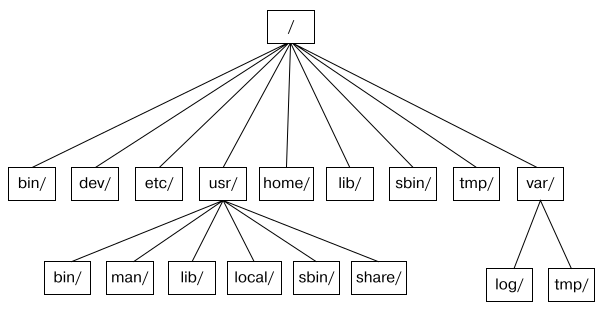
\includegraphics[width=0.85\textwidth]{fhs}
	\caption{Иерархия каталогов Linux}
	\label{fig:fhs}
\end{figure}

\subsection{Описание иерархии каталогов}

К основным каталогам FHS относятся:
\begin{itemize}
	\item \code{/bin/} -- содержит исполняемые файлы, включая большинство основных команд системы UNIX, таких как \code{ls} и \code{cp}.
	\item \code{/boot/} -- содержит файлы загрузчика ядра (данные, которые используются до того, как ядро начинает исполнять программы пользователя).
	\item \code{/dev/} -- содержит файлы устройств.
	\item \code{/etc/} -- содержит конфигурационные файлы и каталоги, специфичные для данной конкретной системы (пароль
	пользователя, файлы загрузки, файлы устройств, сетевые настройки и др.).
	\item \code{/home/} -- содержит личные каталоги обычных пользователей.
	\item \code{/lib/} -- содержит динамические библиотеки, необходимые для работы программ из \code{/bin/}.
	\item \code{/media/} -- является точкой подключения съемных устройств (CD-ROM, флеш-накопители и др.).
	\item \code{/mnt/} -- содержит временно монтируемые файловые системы.
	\item \code{/root/} -- домашний каталог суперпользователя.
	\item \code{/opt/} -- может содержать ПО сторонних разработчиков.
	\item \code{/sbin/} -- содержит основные системные программы для администрирования и настройки системы 
	\item \code{/tmp/} -- предназначен для хранения временных файлов, создаваемых в процессе работы различных программ.(\code{init}, \code{iptables}, \code{ifconfig} и др.).
	\item \code{/usr/} -- вторичная иерархия для данных пользователя,  содержащая разделяемые данные, предназначенные только для чтения:
	\begin{itemize}[topsep=0em]
		\item \code{bin/} -- исполняемые файлы;
		\item \code{include/} -- стандартные заголовочные файлы;
		\item \code{lib/} -- объектные файлы и библиотеки;
		\item \code{local/} -- третичная иерархия для данных, специфичных для данного хоста;
		\item \code{sbin/} -- дополнительные системные программы (демоны различных сетевых сервисов);
		\item \code{share/} -- архитектурно-независимые данные.
	\end{itemize}
	\item \code{/var/} -- содержит файлы с изменяющимися данными: каталоги и файлы логирования (\code{log/}), временные файлы, сохраняемые между перезапусками системы (\code{tmp/}), данные кэшей приложений (\code{cache/}) и др. 
\end{itemize}

\newpage

\section{Типы файлов}

\subsection{Обычные файлы}

К обычным файлам относятся текстовые файлы, изображения, архивы и другие. В утилите \code{ls} обозначается <<\code{-}>>:
\lstinputlisting{1_file_types/file}

\subsection{Каталоги}

Каталоги -- это файлы, в качестве данных которых выступают списки других файлов и каталогов. В утилите \code{ls} обозначается <<\code{d}>>:
\lstinputlisting[deletekeywords={test}]{1_file_types/directory}

\subsection{Символьные ссылки}

Символьная ссылка — это файл в данных которого, содержится указание на адрес другого файла по его имени (но не индексному дескриптору). В утилите \code{ls} обозначается <<\code{l}>>:
\lstinputlisting{1_file_types/symbolic}

\subsection{Файлы устройств}

Файлы устройств -- это файлы, предназначенные для обращения к аппаратному обеспечению компьютера (дискам, принтерам, терминалам и др.). К символьным устройствам обращение происходит последовательно (терминал).
Считывание и запись информации на блочные устройства происходит блоками определенного размера в произвольном порядке (жесткий диск). В утилите \code{ls} обозначаются как <<\code{c}>> и <<\code{d}>> соответственно:
\lstinputlisting[lastline=15]{1_file_types/character}
\lstinputlisting{1_file_types/block}

\subsection{Именованные каналы}

Именованные каналы -- это файлы, позволяющие настроить связь между двумя процессами перенаправив вывод одного процесса на вход другого. Именованный канал позволяет различным процессам обмениваться данными, даже если программы, выполняющиеся в этих процессах, изначально не были написаны для взаимодействия с другими программами. В утилите \code{ls} обозначается <<\code{p}>>:
\lstinputlisting{1_file_types/pipe}

\subsection{Сокеты}

Файлы сокетов -- это файлы, обеспечивающие прямую связь между двумя процессами. Помимо обмена данными, сокеты позволяют обмениваться файловыми дескрипторами. В утилите \code{ls} обозначается <<\code{s}>>:
\lstinputlisting{1_file_types/socket}

\section{Ссылки}

Файлы и директории располагаются на устройстве хранения в виде набора блоков. Информация о файле (такая, как владелец файла, время последнего обращения к файлу, размер файла, права на чтение или запись, является ли элемент файлом или директорией) хранится в индексном дескрипторе \code{inode}. Номер \code{inode}, известный также как порядковый номер файла, является уникальным в пределах отдельной файловой системы. Запись каталога содержит имя файла (или директории), а также указатель на дескриптор inode, в котором хранится информация об этом файле (или директории).

Ссылки -- это просто дополнительные записи каталога, позволяющие обращаться к файлам или директориям по нескольким именам. В Linux существует два типа ссылок на файлы -- \textbf{жесткие} и \textbf{символьные} ссылки. 

\subsection{Жесткие ссылки}

Жесткие ссылки реализованы на более низком уровне файловой системы, чем символьные. Файл размещен только в определенном месте жесткого диска, но на это место могут ссылаться несколько ссылок из файловой системы. Каждая из ссылок -- это отдельный файл, но ведут они к одному участку жесткого диска. Ключевые особенности:
\begin{itemize}
	\item Работают только в пределах одной файловой системы;
	\item Нельзя ссылаться на каталоги;
	\item Имеют ту же информацию \code{inode} и набор разрешений что и у исходного файла;
	\item Разрешения на ссылку изменяться при изменении разрешений файла;
	\item Можно перемещать, переименовывать и удалять файл без вреда ссылке.
\end{itemize}

Создание жестких ссылок и поиск файлов с одинаковым \code{inode}:
\lstinputlisting{2_hardlinks/create}

\subsection{Символические ссылки}

Символические ссылки более всего похожи на обычные ярлыки. Они содержат адрес нужного файла в вашей файловой системе. Когда вы пытаетесь открыть такую ссылку, то открывается целевой файл или папка. Главное ее отличие от жестких ссылок в том, что при удалении целевого файла ссылка останется, но она будет указывать в никуда, поскольку файла на самом деле больше нет. Ключевые особенности:
\begin{itemize}
	\item Могут ссылаться на файлы и каталоги;
	\item Можно ссылаться на другие разделы диска;
	\item Права доступа и номер \code{inode} отличаются от исходного файла;
	\item После удаления, перемещения или переименования файла становятся недействительными;
	\item При изменении прав доступа для исходного файла, права на ссылку останутся неизменными.
\end{itemize}

Создание символьных ссылок:
\lstinputlisting{3_symbolic_links/create}

Рекурсивный поиск всех символьных ссылок на заданный файл в текущей директории:
\lstinputlisting{4_symbolic_links_search/search}

\section{Утилиты работы с файлами}

\subsection{Утилита \code{find}}

\code{find} -- это одна из наиболее важных и часто используемых утилит системы Linux. Это команда для поиска файлов и каталогов на основе специальных условий. Ее можно использовать для поиска файлов по разрешениям (\code{-perm}), владельцам (\code{-user}), группам (\code{-group}), типу (\code{-type}), размеру (\code{-size}) и другим подобным критериям. Кроме того, с найденными файлами можно сразу же выполнять необходимые действия.

Для выполнения произвольных команд для найденных файлов используется опция \code{-exec}. Например, выполнить \code{ls -i} для получения номера \code{inode} каждого файла в текущей директории:
\lstinputlisting{5_find/exec_ls}

Утилите \code{find} можно задать тип искомых файлов. Например, можно найти в текущей директории только символические ссылки и получить более подробную информацию о них с помощью вложенной команды \code{file}.
\lstinputlisting{5_find/links}

\subsection{Утилиты \code{od} и \code{hd}}

Команда \code{od} выдает на стандартный вывод файл в одном или нескольких форматах в соответствии с указанными опциями. При отсутствии опций используется восьмеричный формат (как в опции \code{-o}).
\lstinputlisting{6_od/od}

Команда \code{hd} также может вывести содержимое файла в различных форматах:
\lstinputlisting{6_od/hd}

\section{Права владения и доступа}

\subsection{Файлы \code{/etc/passwd} и \code{/etc/shadow}}

Файл \code{/etc/passwd} содержит список пользователей, которые известны системе. В процессе регистрации пользователя система обращается к этому файлу в поисках идентификатора пользователя и его домашнего каталога. Каждая строка файла описывает одного пользователя и  содержит семь полей, разделенных двоеточиями:
\begin{itemize}
	\item Регистрационное имя;
	\item Зашифрованный пароль или <<заполнитель>> пароля;
	\item Идентификатор пользователя;
	\item Идентификатор группы по умолчанию;
	\item Поле персональных данных;
	\item Домашний каталог;
	\item Командный интерпретатор.
\end{itemize}

Примеры строк, хранящихся в \code{/etc/passwd}:
\lstinputlisting{7_access/passwd}

Файл \code{/etc/shadow} доступен для чтения только пользователю root и предназначен для хранения зашифрованных паролей. В нем также содержится учетная информация, которая отсутствует в файле \code{/etc/passwd}. При использовании скрытых паролей соответствующие поля в файле \code{/etc/passwd} всегда содержат символ «\code{х}». Каждая строка состоит из 9 полей, разделенных двоеточиями:
\begin{itemize}
	\item Регистрационное имя;
	\item Зашифрованный пароль;
	\item Дата последнего изменения пароля;
	\item Минимальное число дней между изменениями пароля;
	\item Максимальное число дней между изменениями пароля;
	\item Количество дней до истечения срока действия пароля, когда выдается предупреждение;
	\item Количество дней по истечении срока действия пароля, когда учетная запись отключается;
	\item Срок действия учетной записи;
	\item Зарезервированное поле, которое в настоящее время всегда пустое.
\end{itemize}

Пример записи о пользователе в \code{/etc/shadow}:
\lstinputlisting{7_access/shadow}

\subsection{Права владения}

Файлы в UNIX имеют двух владельцев: пользователя и группу. Пользователь-владелец может не являться членом группы-владельца. Владельцем-пользователем вновь созданного файла является пользователь, создавший файл. Права владения отображаются в третьей и четвертой колонке при выполнении команды \code{ls -l}:
\lstinputlisting[lastline=3]{7_access/chown}

Для изменения владельца используется команда \code{chown}. Например, можно сменить владельца-пользователя и владельца-группу на \code{root}:
\lstinputlisting[firstline=4]{7_access/chown}

\subsection{Права доступа}

В операционной системе UNIX существуют три базовых класса доступа к файлу, в каждом из которых установлены соответствующие права доступа:
\begin{itemize}
	\item User access (\code{u}) -- для пользователя-владельца файла;
	\item Group access (\code{g}) -- для членов группы, являющейся владельцем файла;
	\item Other access (\code{о}) -- для остальных пользователей (кроме root).
\end{itemize}

ОС UNIX поддерживает три типа прав доступа для каждого класса: 
\begin{itemize}
	\item на чтение (Read, \code{г});
	\item на запись (Write, \code{w});
	\item на выполнение (eXecute, \code{х}).
\end{itemize}

Права доступа отображаются в первой колонке при выполнении команды \code{ls -l} (кроме первого символа):
\lstinputlisting{7_access/ls}

Права доступа могут быть изменены только владельцем файла или root с помощью команды \code{chmod}. Например можно дать право на запись членам группы владельца:
\lstinputlisting[lastline=7]{7_access/chmod}

Дать право на выполнение всем трем группам:
\lstinputlisting[firstline=8, lastline=11]{7_access/chmod}

Забрать право на выполнение у остальных пользователей:
\lstinputlisting[firstline=12]{7_access/chmod}

Сменить владельца и группу владельца файла:
\lstinputlisting{7_access/chown}

\subsection{Атрибуты \code{SUID} и \code{SGID}}

Существуют другие атрибуты, изменяющие стандартное выполнение программ. Например, Set UID/SUID; Set GID/SGID (\code{s}) установают UID или GID процесса при выполнении.

Атрибуты \code{SUID} и \code{SGID} позволяют изменить права пользователя при запуске на выполнение файла, имеющего эти атрибуты. При этом привилегии будут изменены (обычно расширены) лишь на время выполнения и только в отношении этой программы.

Обычно запускаемая программа получает права доступа к системным ресурсам на основе прав доступа пользователя, запустившего программу. Установка флагов \code{SUID} и \code{SGID} изменяет это правило, назначая права доступа исходя из прав доступа владельца файла. Таким образом, запущенный исполняемый файл, которым владеет суперпользователь, получает неограниченные права доступа к системным ресурсам, независимо от того, кто его запустил.

Примером файла с таким атрибутом является утилита \code{passwd(1)}, позволяющая пользователю поменять пароль:
\lstinputlisting{7_access/suid}

Изменение пароля должно приводить к изменению файлов \code{/etc/passwd} и \code{/etc/shadow}. Но вместо того, чтобы давать возможность записи в эти файлы всем пользователям, программа \code{/usr/bin/passwd}, владельцем которой является \code{root}, содержит флаг \code{SUID}. Таким образом, любой пользователь, запускающий утилиту \code{passwd}, получает на время выполнения права суперпользователя.

% \subsection{Программа-шлюз}

\section{Утилиты получения информации о ФС}

\subsection{Утилита \code{df}}

Утилита \code{df} (disk free) выводит список всех файловых систем по именам устройств с указанием размера, показывает точки монтирования и количество свободного/занятого пространства.
\lstinputlisting{8_fs/df}

В выводе отображается информация как о реальных, так и виртуальных файловых системах. Для вывода данных только о реальных файловых системах используется команда:
\lstinputlisting{8_fs/df_real}


\subsection{Файл \code{/etc/fstab}}

Файл \code{/etc/fstab} -- это текстовый файл, который содержит информацию о различных файловых системах и устройствах хранения информации в вашем компьютере. Это всего лишь один файл, определяющий, как диск и/или раздел будут использоваться и как будут встроены в остальную систему. 

Этот файл можно открыть в любом текстовом редакторе, но редактировать его возможно только от имени суперпользователя, т.к. файл является важной, неотъемлемой частью системы, без него система не загрузится. При загрузке операционной системы, \code{fsck} считывает список монтируемых файловых систем из файла \code{/etc/fstab}.

\lstinputlisting{8_fs/fstab}

Строки файла содержат следующие поля:
\begin{itemize}
	\item Что монтируем -- некоторое блочное устройство, которое должно быть примонтировано;
	\item Куда монтируем -- точка монтирования - путь в корневой файловой системе к каталогу в который будет смонтировано устройство;
	\item Тип файловой системы монтируемого раздела;
	\item Опции монтирования файловой системы;
	\item Индикатор необходимости делать резервную копию (как правило не используется и равно 0);
	\item Порядок проверки раздела (0 -- не проверять, 1 -- устанавливается для корня, 2 -- для остальных разделов).
\end{itemize}

\subsection{Утилита \code{file}}

\section{Выводы}

В процессе выполнения данной работы:
\begin{itemize}
	\item Вывод
	\item Вывод
\end{itemize}


\end{document}
